\subsubsection{Problem 2}
\textbf{Observability Analysis}\\
From the system matrix in \eqref{p4_sys_AB} and the output matrix in \eqref{p4_sys_C}, the observability matrix can be found to be
\begin{equation}
    \setstackgap{L}{1.1\baselineskip}
    \fixTABwidth{T}
    \mathbf{\mathcal{O}} = 
        \begin{bmatrix}
        \mathbf{C}      \\
        \mathbf{CA}     \\
        \mathbf{CA^2}   \\
        \mathbf{CA^3}   \\
        \mathbf{CA^4}   \\
        \mathbf{CA^5}   \\
    \end{bmatrix}
    =
    \bracketMatrixstack{
    1       & 0       & 0 & 0 & 0 & 0 \\
    0       & 0       & 1 & 0 & 0 & 0 \\
    0       & 0       & 0 & 0 & 1 & 0 \\
    0       & 1       & 0 & 1 & 0 & 0 \\
    0       & 0       & 0 & 0 & 0 & 1 \\
    0       & 0       & 0 & 0 & 0 & 0 \\
    0       & 0       & 0 & 0 & 0 & 0 \\
    -0.612  & 0       & 0 & 0 & 0 & 0 \\
    0       & 0       & 0 & 0 & 0 & 0 \\
    0       & 0       & 0 & 0 & 0 & 0 \\
    0       & -0.612  & 0 & 0 & 0 & 0 \\
    0       & 0       & 0 & 0 & 0 & 0 \\
    0       & 0       & 0 & 0 & 0 & 0 \\
    0       & 0       & 0 & 0 & 0 & 0 \\
    0       & 0       & 0 & 0 & 0 & 0 \\
    0       & 0       & 0 & 0 & 0 & 0 \\
    0       & 0       & 0 & 0 & 0 & 0 }
    \text{.}
\end{equation}
The matrix has full column rank, which means the system is observable.\\\\
\textbf{Linear Observer Design}\\
We wish to control the system using an estimated state $\mathbf{\hat{x}}$. A \textit{linear observer} (or closed-loop estimator) is then
\begin{equation}
    \label{eq:observer}
    \mathbf{\dot{\hat{x}}} = \mathbf{A\hat{x}} + \mathbf{Bu} + \mathbf{L} (\mathbf{y} - \mathbf{C\hat{x}}),
\end{equation}
where $\mathbf A$, $\mathbf B$ and $\mathbf C$ are as before and $\mathbf L$ is the \textit{observer gain matrix}. \\
Replacing the output with $\mathbf{C}\mathbf{x}$ and rearranging yields
\begin{equation*}
   \mathbf{\dot{\hat{x}}} = (\mathbf{A} - \mathbf{LC})(\mathbf{\hat{x}} - \mathbf{x}) + \mathbf{Ax} + \mathbf{LC}(\mathbf{x} - \mathbf{\hat{x}}),
\end{equation*}
and when inserting the estimation error (denoted $\mathbf{d}$ as in \textit{deviation} here, to not confuse it with the elevation $e$), 
\begin{equation}
    \mathbf{d} = \hat{\mathbf{x}} - \mathbf{x} \label{eq:est_error},
\end{equation}
along with its derivative, the observer's error dynamics, become
\begin{equation}
    \mathbf{\dot{d}} = (\mathbf{A} - \mathbf{LC})\mathbf{d}. \label{eq:observer_error_sys}
\end{equation}
Good state estimation is essential to properly control the helicopter. The error dynamics of the observer thus need to be faster than the dynamics of the feedback controller. This corresponds to the poles of the closed loop observer being more \textit{negative} than the controller poles. Conveniently, by theorem 8.O3 in Chen, the poles of the closed loop observer, i.e. the eigenvalues of $\mathbf{A} - \mathbf{LC}$, can be placed arbitrarily with appropriate choice of observer gain $\mathbf{L}$.\cite{Chen2014}

To place the poles like so, one can use the matlab \texttt{place} command. This command will output a feedback gain matrix that will place the poles of a closed loop system at the values given in a vector $\mathbf{p}$.
This applies to using a feedback controller such as $\mathbf{u} = -\mathbf{Kx}$. In that case, the closed loop dynamics of the system, $\mathbf{\dot{x}} = \mathbf{Ax} + \mathbf{Bu}$, will be
\begin{equation*}
    \mathbf{\dot{x}} = (\mathbf{A} - \mathbf{BK})\mathbf{x}.
\end{equation*}
 Using the  matlab \texttt{place} command as such:
\begin{verbatim}
    K = place(A, B, p);
\end{verbatim}
will produce a feedback gain matrix $\mathbf{K}$, that places the eigenvalues of $\mathbf{A} - \mathbf{BK}$ at the desired values.\cite{MathWorks2018}

For the closed loop observer in \eqref{eq:observer}, the only modifiable matrix is $\mathbf{L}$. By the properties of the transpose, 
\begin{equation*}
    (\mathbf{A} - \mathbf{LC})^\text{T} = \mathbf{A}^\text{T} - (\mathbf{LC})^\text{T} = \mathbf{A}^\text{T} - \mathbf{C}^\text{T} \mathbf{L}^\text{T},
\end{equation*}
such that
\begin{equation*}
    \mathbf{L}^\text{T} = \texttt{Place}(\mathbf{A}^\text{T}, \mathbf{C}^\text{T}, \mathbf{p}).
\end{equation*}
And so finally, by the property that any matrix has eigenvalues identical to its transpose, the required matrix can be calculated as
\begin{equation}
    \label{eq:est_pole_place}
    \mathbf{L} = \texttt{Place}(\mathbf{A}^\text{T}, \mathbf{C}^\text{T}, \mathbf{p})^\text{T},
\end{equation}
where the desired eigenvalues are given in the vector $\mathbf{p}$.\\
Furthermore, by substituting the estimate $\mathbf{\hat{x}}$ for $\mathbf{x}$ in the feedback controller $\mathbf{u} = -\mathbf{Kx}$ from problem 3, the estimated system becomes
\begin{equation}
    \mathbf{\dot{\hat{x}}} = (\mathbf{A} - \mathbf{LC} - \mathbf{BK})\mathbf{\hat{x}} - \mathbf{L} \mathbf{y}.
\end{equation}
Thus, the dynamics of the closed loop system, with controller and estimator are 
\begin{align}
    \begin{bmatrix}
    \mathbf{\dot{x}} \\
        \mathbf{\dot{d}}
        \end{bmatrix}
    = \begin{bmatrix}
        \mathbf{A} - \mathbf{BK} & \mathbf{BK} \\
        \mathbf{0}               & \mathbf{A} - \mathbf{LC}
    \end{bmatrix}
    \begin{bmatrix}
        \mathbf{x} \\
        \mathbf{d}
    \end{bmatrix}.
\end{align}
Note how, since this matrix is triangular, its eigenvalues are simply those of the diagonal matrices. The stability of the entire system can hence be determined by verifying stability in the observer and the system separately,\cite{StackExchange} a principle known as the \textit{separation principle}.\cite{Chen2014}\\\\
\textbf{Observer Tuning}\\
By the separation principle, tuning of the observer can be done independently of the controller. However, as mentioned previously, the poles of the observer should be placed much further to the left in the complex plane than the poles of the closed loop feedback controller. With the \texttt{place} command, the poles are placed in a fan as illustrated in figure \ref{fig:P4p2_observer_poles}.
\begin{figure}[htb]
    \begin{minipage}{0.5\textwidth}
    	\centering
    	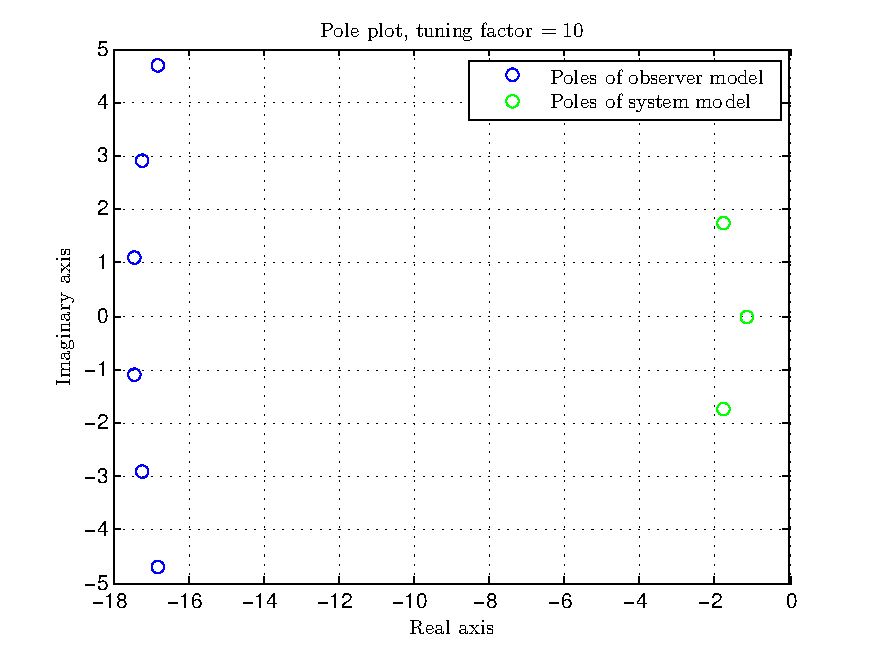
\includegraphics[width=1\textwidth,trim={0cm 0cm 0cm 0cm},clip]{figures/P4p2_pole_plot_tuning_factor_10.pdf}
    	\caption{Observer and system poles}
        \label{fig:P4p2_observer_poles}
    \end{minipage}
    \begin{minipage}{0.5\textwidth}
        \centering
    	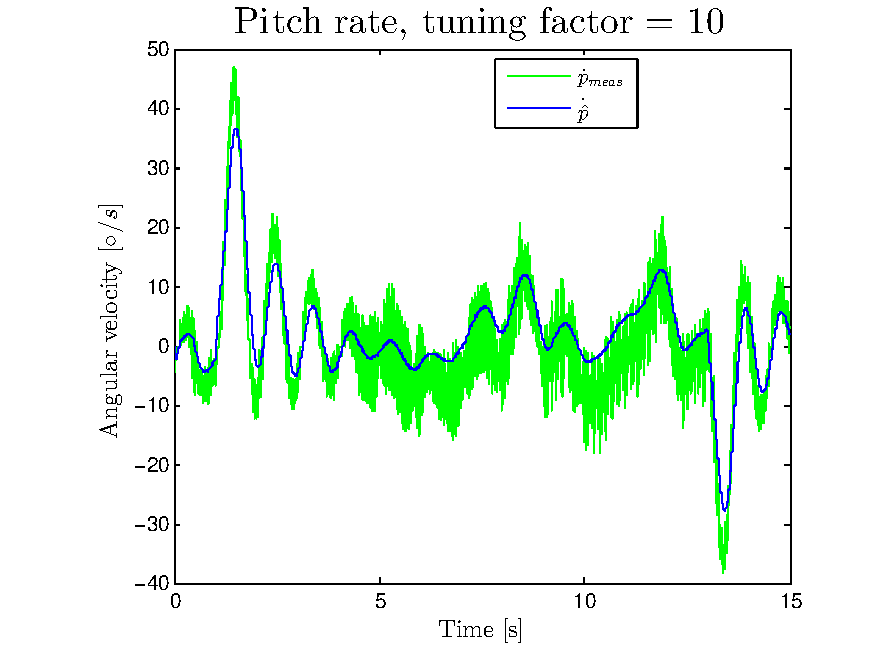
\includegraphics[width=1\textwidth,trim={0cm 0cm 0cm 0cm},clip]{figures/P4p2_pitch_rate_tuning_factor_10.pdf}.
    	\caption{Pitch rate with timid observer}
        \label{fig:P4p2_pitch_rate_10}
    \end{minipage}
\end{figure}
Having the poles be quite negative as they are here, makes the observer fast and easily able to track the state closely, neither does it introduce any noticeable lag or instability into the system.

An example plot showing the estimated pitch rate, $\dot{\hat{p}}$ (in blue) and the measured state (in green) are shown in figure \ref{fig:P4p2_pitch_rate_10}, which confirms these assumptions. The only considerable estimation error appears in the pitch rate, when the helicopter turns quickly. This is likely caused by the pitch rate being so far from zero, which is the value it was linearized around. Had the other two estimates, elevation rate and travel rate, displayed similar behaviour, estimation errors would probably appear there too. However, since the states are so much slower, this is not the case.

The poles in this case were placed around $-17$. This makes the observer fast enough for this application, but not fast enough to track the state perfectly. This slowness also has the side effect of low-pass filtering the response, which makes for clear looking plots. 

Nevertheless, it can be useful to make the poles even more negative. Placing them at around $-250$ for instance, makes the response very noisy, but with very close tracking of the actual state, as can be shown in figure \ref{fig:P4p2_travel_rate_150}.

\begin{figure}[htb]
	\centering
		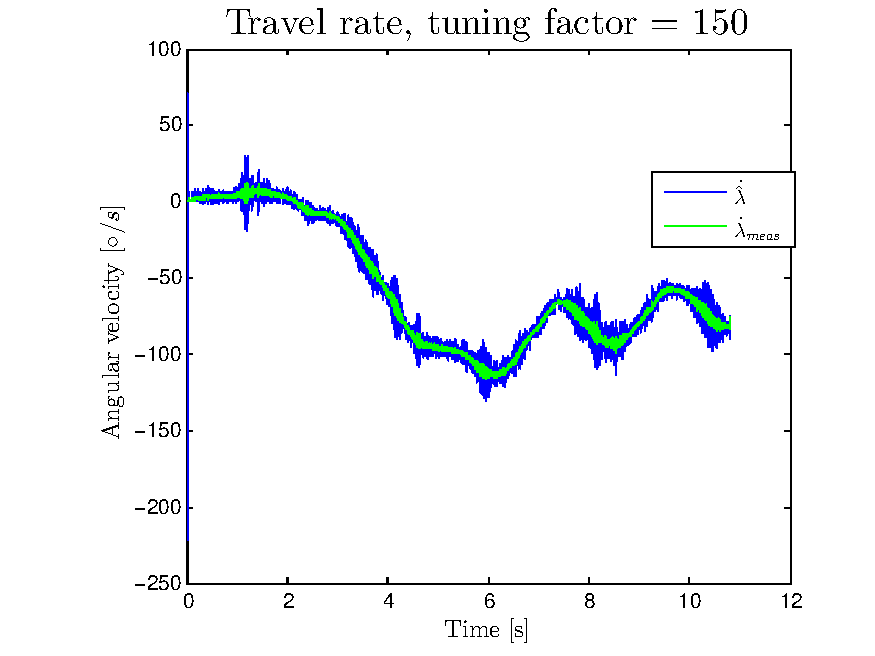
\includegraphics[width=0.6\textwidth,trim={0cm 0cm 0cm 0cm},clip]{figures/P4p2_travel_rate_tuning_factor_150_OLD.pdf}.
	\caption{Travel rate with very fast observer}
\label{fig:P4p2_travel_rate_150}
\end{figure}
It is in fact easy to show that very negative eigenvalues of $\mathbf{L}$ scale up any unwanted measurement measurement noise heavily, just like in this case. Rewriting \eqref{eq:observer} with $\mathbf{y} = \mathbf{Cx} + \mathbf{w}$ as output, where the vector $\mathbf{w}$ represents the measurement noise in the output, means \eqref{eq:observer_error_sys} instead becomes
\begin{equation}
    \mathbf{\dot{d}} = (\mathbf{A} - \mathbf{LC})\mathbf{d} - \mathbf{Lw}.
\end{equation}
An $\mathbf{L}$ matrix with very negative eigenvalues will thus result in $|\mathbf{Lw}|$ becoming very large and introduce high amplitude noise into the estimation error dynamics. 

A middle ground, with poles placed around $-120$, results in precise estimation of the measured value. It introduces a bit of noise, but no more than their measured counterparts do. Plots that show how well the estimated states, $\dot{\hat{p}}$, $\dot{\hat{e}}$ and $\dot{\hat{\lambda}}$ compare to the measured states, are shown in figures \ref{fig:P4p2_pitch_rate_70}, \ref{fig:P4p2_elevation_rate_70} and \ref{fig:P4p2_travel_rate_70}, respectively. The pole placement is shown in figure \ref{fig:P4p2_pole_plot_70} 
\begin{figure}[htb]
    \begin{minipage}{0.5\textwidth}
    	\centering
    	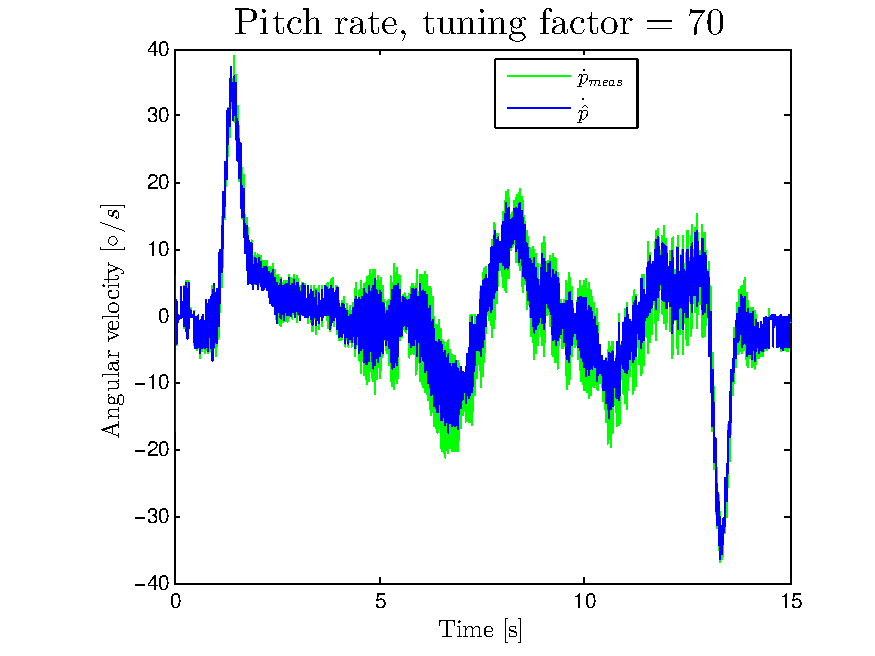
\includegraphics[width=1\textwidth,trim={0cm 0cm 0cm 0cm},clip]{figures/P4p2_pitch_rate_tuning_factor_70.pdf}
    	\caption{Pitch rate with moderate estimator}
        \label{fig:P4p2_pitch_rate_70}
    \end{minipage}    
    \begin{minipage}{0.5\textwidth}
    	\centering
		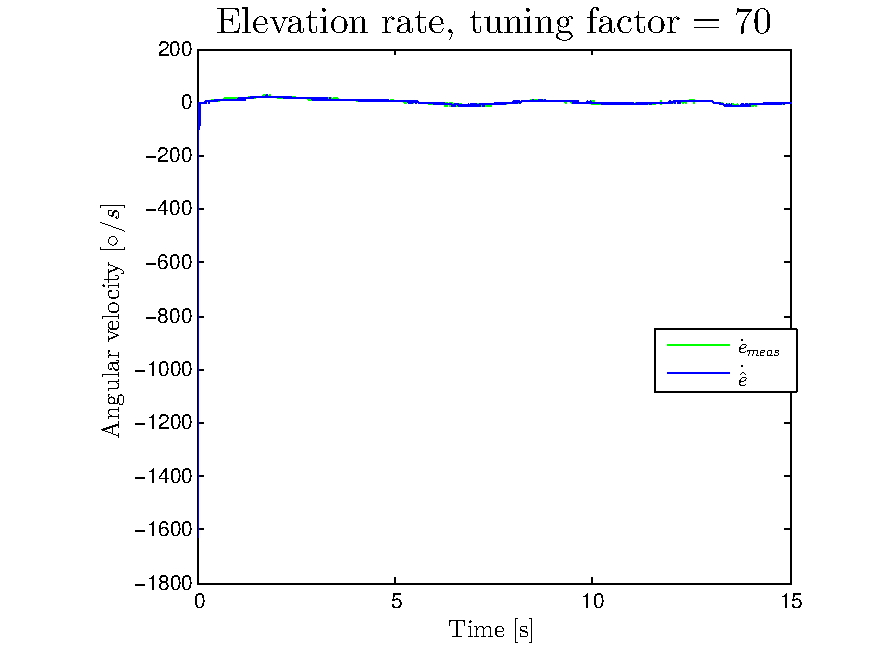
\includegraphics[width=1\textwidth,trim={0cm 0cm 0cm 0cm},clip]{figures/P4p2_elevation_rate_tuning_factor_70.pdf}
    	\caption{Elevation rate with moderate estimator}
    \label{fig:P4p2_elevation_rate_70}
    \end{minipage}    
\end{figure}
\begin{figure}[htb]
    \begin{minipage}{0.5\textwidth}
    	\centering
		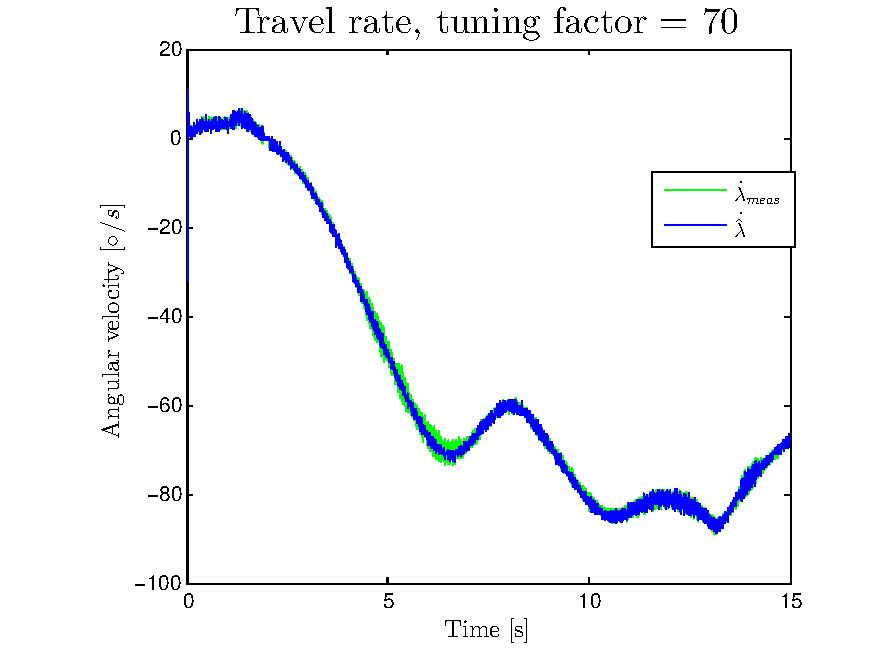
\includegraphics[width=1\textwidth,trim={0cm 0cm 0cm 0cm},clip]{figures/P4p2_travel_rate_tuning_factor_70.pdf}
    	\caption{Travel rate with moderate observer}
        \label{fig:P4p2_travel_rate_70}
    \end{minipage}    
    \begin{minipage}{0.5\textwidth}
    	\centering
		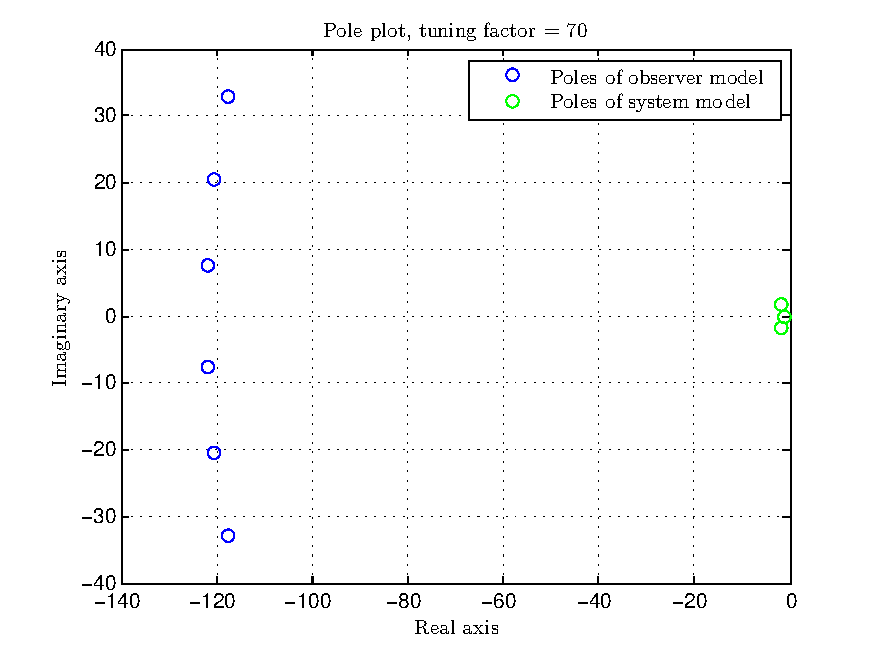
\includegraphics[width=1\textwidth,trim={0cm 0cm 0cm 0cm},clip]{figures/P4p2_pole_plot_tuning_factor_70.pdf}
    	\caption{Pole plot with moderate observer}
        \label{fig:P4p2_pole_plot_70}
    \end{minipage}    
\end{figure}